\ifx\wholebook\relax \else
% ------------------------

\documentclass[UTF8]{article}
%------------------- Other types of document example ------------------------
%
%\documentclass[twocolumn]{IEEEtran-new}
%\documentclass[12pt,twoside,draft]{IEEEtran}
%\documentstyle[9pt,twocolumn,technote,twoside]{IEEEtran}
%
%-----------------------------------------------------------------------------
%
% loading packages
%

\RequirePackage{ifpdf}
\RequirePackage{ifxetex}

%
%
\ifpdf
  \RequirePackage[pdftex,%
       bookmarksnumbered,%
              colorlinks,%
          linkcolor=blue,%
              hyperindex,%
        plainpages=false,%
       pdfstartview=FitH]{hyperref}
\else\ifxetex
  \RequirePackage[bookmarksnumbered,%
               colorlinks,%
           linkcolor=blue,%
               hyperindex,%
         plainpages=false,%
        pdfstartview=FitH]{hyperref}
\else
  \RequirePackage[dvipdfm,%
        bookmarksnumbered,%
               colorlinks,%
           linkcolor=blue,%
               hyperindex,%
         plainpages=false,%
        pdfstartview=FitH]{hyperref}
\fi\fi
%\usepackage{hyperref}

% other packages
%--------------------------------------------------------------------------
\usepackage{graphicx, color}
\usepackage{subfig}
\usepackage{multicol}
\usepackage{tikz}
\usetikzlibrary{matrix,positioning,shapes}

\usepackage{amsmath, amsthm, amssymb} % for math
\usepackage{exercise} % for exercise
\usepackage{import} % for nested input

%
% for programming
%
\usepackage{verbatim}
\usepackage{fancyvrb}
\usepackage{listings}
%\usepackage{algorithmic} %old version; we can use algorithmicx instead
%\usepackage[plain]{algorithm} %remove rule (horizontal line on top/below the algorithm
\usepackage{algorithm} %to remove rules change to \usepackage[plain]{algorithm}
%\usepackage{algorithm2e}
\usepackage[noend]{algpseudocode} %for pseudo code, include algorithmicsx automatically
\usepackage{appendix}
\usepackage{makeidx} % for index support
\usepackage{titlesec}

\usepackage[cm-default]{fontspec}
\usepackage{xunicode}
%\usepackage{fontenc}
\usepackage{textcomp}
\usepackage{url}

% detect and select Chinese font
% ------------------------------
% the following cmd can list all availabe Chinese fonts in host.
% fc-list :lang=zh
\def\myfont{STSong}  % Under Mac OS X
\def\linuxfallback{WenQuanYi Micro Hei} % Under Linux
\def\winfallback{SimSun} % Under Windows
\suppressfontnotfounderror1 % Avoid setting exit code (error level) to break make process
\count255=\interactionmode
\batchmode
\font\foo="\myfont"\space at 10pt
\ifx\foo\nullfont
  \font\foo = "\linuxfallback"\space at 10pt
  \ifx\foo\nullfont
    \font\foo = "\winfallback"\space at 10pt
    \ifx\foo\nullfont
      \errorstopmode
      \errmessage{no suitable Chinese font found}
    \else
      \let\myfont=\winfallback % Windows
    \fi
  \else
    \let\myfont=\linuxfallback % Linux
  \fi
\fi
\interactionmode=\count255
\setmainfont[Mapping=tex-text]{\myfont}
\setmonofont[Scale=MatchLowercase]{Monaco}   % 英文等宽字体

\XeTeXlinebreaklocale "zh"  % to solve the line breaking issue
\XeTeXlinebreakskip = 0pt plus 1pt minus 0.1pt

\titleformat{\paragraph}
{\normalfont\normalsize\bfseries}{\theparagraph}{1em}{}
\titlespacing*{\paragraph}
{0pt}{3.25ex plus 1ex minus .2ex}{1.5ex plus .2ex}

\lstdefinelanguage{Smalltalk}{
  morekeywords={self,super,true,false,nil,thisContext}, % This is overkill
  morestring=[d]',
  morecomment=[s]{"}{"},
  alsoletter={\#:},
  escapechar={!},
  literate=
    {BANG}{!}1
    {UNDERSCORE}{\_}1
    {\\st}{Smalltalk}9 % convenience -- in case \st occurs in code
    % {'}{{\textquotesingle}}1 % replaced by upquote=true in \lstset
    {_}{{$\leftarrow$}}1
    {>>>}{{\sep}}1
    {^}{{$\uparrow$}}1
    {~}{{$\sim$}}1
    {-}{{\sf -\hspace{-0.13em}-}}1  % the goal is to make - the same width as +
    %{+}{\raisebox{0.08ex}{+}}1		% and to raise + off the baseline to match -
    {-->}{{\quad$\longrightarrow$\quad}}3
	, % Don't forget the comma at the end!
  tabsize=2
}[keywords,comments,strings]

% for literate Haskell code
\lstdefinestyle{Haskell}{
  flexiblecolumns=false,
  basewidth={0.5em,0.45em},
  morecomment=[l]--,
  literate={+}{{$+$}}1 {/}{{$/$}}1 {*}{{$*$}}1 {=}{{$=$}}1
           {>}{{$>$}}1 {<}{{$<$}}1 {\\}{{$\lambda$}}1
           {\\\\}{{\char`\\\char`\\}}1
           {->}{{$\rightarrow$}}2 {>=}{{$\geq$}}2 {<-}{{$\leftarrow$}}2
           {<=}{{$\leq$}}2 {=>}{{$\Rightarrow$}}2
           {\ .}{{$\circ$}}2 {\ .\ }{{$\circ$}}2
           {>>}{{>>}}2 {>>=}{{>>=}}2
           {|}{{$\mid$}}1
}

\lstloadlanguages{C, C++, Lisp, Haskell, Python, Smalltalk}

\lstset{
  basicstyle=\small\ttfamily,
  commentstyle=\rmfamily,
  texcl=true,
  showstringspaces = false,
  upquote=true,
  flexiblecolumns=false
}

% ======================================================================

\def\BibTeX{{\rm B\kern-.05em{\sc i\kern-.025em b}\kern-.08em
    T\kern-.1667em\lower.7ex\hbox{E}\kern-.125emX}}

%
% mathematics
%
\newcommand{\be}{\begin{equation}}
\newcommand{\ee}{\end{equation}}
\newcommand{\bmat}[1]{\left( \begin{array}{#1} }
\newcommand{\emat}{\end{array} \right) }
\newcommand{\VEC}[1]{\mbox{\boldmath $#1$}}

% numbered equation array
\newcommand{\bea}{\begin{eqnarray}}
\newcommand{\eea}{\end{eqnarray}}

% equation array not numbered
\newcommand{\bean}{\begin{eqnarray*}}
\newcommand{\eean}{\end{eqnarray*}}

\newtheorem{theorem}{定理}[section]
\newtheorem{lemma}[theorem]{引理}
\newtheorem{proposition}[theorem]{Proposition}
\newtheorem{corollary}[theorem]{Corollary}

% 中文书籍设置
% ====================================
\renewcommand\contentsname{目\ 录}
%\renewcommand\listfigurename{插图目录}
%\renewcommand\listtablename{表格目录}
\renewcommand\figurename{图}
\renewcommand\tablename{表}
\renewcommand\proofname{证明}
\renewcommand\ExerciseName{练习}
%\renewcommand{\algorithmcfname}{算法}

\ifx\wholebook\relax
\renewcommand\bibname{参\ 考\ 文\ 献}                    %book类型
%\newtheorem{Definition}[Theorem]{定义}
\newtheorem{Theorem}{定理}[chapter]
\newtheorem{example}{例题}[chapter]
\else
\renewcommand\refname{参\ 考\ 文\ 献}
\fi

%\setcounter{secnumdepth}{4}
\titleformat{\chapter}
  {\normalfont\bfseries\Large}
  {第\arabic{chapter}章}
  {12pt}{\Large}
%% \titleformat{\subsection}
%%   {\normalfont\bfseries\large}
%%   {\CJKnumber{\arabic{subsection}}、}
%%   {12pt}{\large}
%% \titleformat{\subsubsection}
%%   {\normalfont\bfseries\normalsize}
%%   {\arabic{subsubsection}.}
%%   {12pt}{\normalsize}

%\renewcommand{\baselinestretch}{1.5}                        %文章行间距为1.5倍。

\makeatletter
\newcommand{\verbatimfont}[1]{\renewcommand{\verbatim@font}{\ttfamily#1}}
\makeatother

\setcounter{tocdepth}{4}
\setcounter{secnumdepth}{4}

%\verbatimfont{\footnotesize}


\setcounter{page}{1}

\begin{document}

%--------------------------

% ================================================================
%                 COVER PAGE
% ================================================================

\title{基数树-Trie和前缀树}

\author{刘新宇
\thanks{{\bfseries 刘新宇 } \newline
  Email: liuxinyu95@gmail.com \newline}
  }

\maketitle
\fi

\markboth{基数树-Trie和前缀树}{初等算法}

\ifx\wholebook\relax
\chapter{基数树-Trie和前缀树}
\numberwithin{Exercise}{chapter}
\fi

%{\bfseries Corresponding Author:} Larry LIU Xinyu


% ================================================================
%                 Introduction
% ================================================================
\section{简介}
\label{introduction}
\index{基数树}

前面章节介绍的各种树都是利用节点来存储信息,我们也可以利用边(edge)来存储。基数树(Radix tree),如Trie和前缀树就是这样的数据结构。它们产生于1960年代,被广泛用于编译器\cite{okasaki-int-map}和生物信息处理(如DNA模式匹配)\cite{wiki-suffix-tree}等领域。

\begin{figure}[htbp]
  \centering
  \includegraphics[scale=0.4]{img/radix-tree.ps}
  \caption{基数树} \label{fig:radix-tree}
\end{figure}

图\ref{fig:radix-tree}展示了一棵基数树(\cite{CLRS}第269页)。它包含了串1011、10、011、100和0。如果要在其中查找二进制数$k=(b_0b_1...b_n)_2$,我们首先检查左侧的最高位$b_0$是1还是0,若为0,则接下来在左侧分支查找;若为1,则继续在右侧分支查找。接着,我们检查第二位,并重复这一过程直到处理完所有的$n$位或到达某一叶子节点。

基数树并不在节点中存储key,信息由边来代表。图中节点中标注的key仅仅是为了方便理解。使用整数的二进制串来代表key,既可以节省空间,又可以通过位运算,加快处理速度。

% ================================================================
%                 Int Trie
% ================================================================
\section{整数Trie}
\label{int-trie}
\index{基数树!整数trie}

图\ref{fig:radix-tree}中所示的数据结构常被称为\emph{binary trie}。Trie是Edward Fredkin提出的。它来自英文单词retrieval,最开始发音为/'tri:/。但是许多人都把它读作/'trai/(和英文单词try的发音相同)\cite{wiki-trie}。Trie也被称为前缀树。一棵binary trie是一种特殊的二叉树,每个key存放的位置由它的二进制位来决定。0表示“向左”,而1表示“向右”\cite{okasaki-int-map}。

由于整数可以表示为二进制,我们可以用整数代替0/1串作为key。当把一个整数插入到Trie时,我们首先将其转化为二进制,然后检查第一位,若为0,则递归插入到左侧分支,若为1,则插入到右侧分支。但是这里有一个问题。考虑图\ref{fig:big-endian-trie}中的Trie,如果使用0/1串,这3个key各不相同,但它们却代表同一个十进制整数。对于这个例子来说,我们应该在Trie中的哪个位置插入整数3呢?

\begin{figure}[htbp]
  \centering
  \includegraphics[scale=0.4]{img/big-endian-trie.ps}
  \caption{大端(big-endian)Trie} \label{fig:big-endian-trie}
\end{figure}

如果把前面的0也当作有效位,在一个32位整数的系统中,向空Trie插入1,结果将是一棵有32层分支的树。其中的31个中间节点只有一个左子树,最后一个节点只有一个右子树。空间利用率很低。

Okasaki给出了一种解决方法\cite{okasaki-int-map}。二进制数的最高位(MSB)通常在左边,最低位(LSB)在右边。这种Trie称作大端(big-endian)树。我们也可以使用小端(little-endian)数来表示key。这样,十进制的1表示为小端二进制的1。如果插入到空Trie中,结果就是含有一个右侧叶子节点的树。它只有一层分支。十进制的2将被表示为小端二进制的01,十进制的3表示为小端二进制$(11)_2$。这样就消除了有效位前面的0,每一个整数key在Trie中的位置可以被唯一确定。

%=========================================================================
%       Definition of integer trie
%=========================================================================
\subsection{整数Trie的定义}
我们可以重用二叉树的结构来定义binary trie。一个binary trie的节点要么为空,要么包含左右两个分支。非空节点可以保存额外的附加数据(satellite data)。左侧分支编码为0,右侧分支编码为1。

下面的Scala例子代码定义了Trie的代数数据类型。

\lstset{language=Scala}
\begin{lstlisting}
sealed trait IntTrie[+A]
case object Empty extends IntTrie[Nothing]
case class Br[A] (left: IntTrie[A],
                  value: Option[A],
                  right: IntTrie[A]) extends IntTrie[A]
\end{lstlisting}

在命令式编程语言中,Trie通常被定义为结构或类,如下面的Java例子代码所示:

\lstset{language=Java}
\begin{lstlisting}
public class Node<T> {
    T value;
    Node<T> left;
    Node<T> right;

    public Node(T val) { value = val; }
    public Node() { this(null); }
}
\end{lstlisting}


% ================================================================
%               Insertion of integer trie
% ================================================================
\subsection{插入}
\index{整数trie!插入}

由于整数Trie的定义是递归的,插入算法可以很自然地用递归进行定义。如果最左侧的位为0,说明待插入的key为偶数,我们接下来在左侧分支递归插入;否则最左侧的位为1,说明key为奇数,我们转向右侧分支。我们这样不断地将key除以2取整以去掉最左侧的位,直到处理完所有的位。此时key变为0,插入结束。记Trie树$T$的左右分支为$T_l$和$T_r$,节点上存储的数据为$d$(可以为空)。如果$T$为空,则其左右分支和数据也定义为空。我们可以这样定义插入算法:

\be
insert(T, k, v) = \left \{
  \begin{array}
  {r@{\quad:\quad}l}
  (T_l, v, T_r) & k = 0 \\
  (insert(T_l, k / 2, v), d, T_r) & even(k) \\
  (T_l, d, insert(T_r, \lfloor k / 2 \rfloor, v)) & otherwise
  \end{array}
\right.
\ee

如果待插入的key已经存在,这一算法会覆盖原来存储的数据。也可以使用链表保存同一key上的所有数据。

图\ref{int-trie}的例子是依次插入射对\{$ 1 \rightarrow a, 4 \rightarrow b, 5 \rightarrow c, 9 \rightarrow d$\}的结果。

\begin{figure}[htbp]
  \centering
  \includegraphics[scale=0.5]{img/int-trie.ps}
  \caption{用小端整数binary trie实现的映射:
          \{$ 1 \rightarrow a, 4 \rightarrow b, 5 \rightarrow c, 9 \rightarrow d$\}}
  \label{fig:int-trie}
\end{figure}

下面的Scala例子程序实现了这一插入算法。

\lstset{language=Scala}
\begin{lstlisting}
def insert[A] (t: IntTrie[A], key: Int, value: A): IntTrie[A] = {
  val l = left(t)
  val r = right(t)
  val v = getValue(t)
  if (key == 0) {
    Br(l, Some(value), r)
  } else if (key % 2 == 0) {   //even
    Br(insert(l, key / 2, value), v, r)
  } else {
    Br(l, v, insert(r, key / 2, value))
  }
}

def left[A] (t: IntTrie[A]): IntTrie[A] = t match {
  case Empty => Empty
  case Br(l, _, _) => l
}

def right[A] (t: IntTrie[A]): IntTrie[A] = t match {
  case Empty => Empty
  case Br(_, _, r) => r
}

def getValue[A] (t: IntTrie[A]): Option[A] = t match {
  case Empty => None
  case Br(_, v, _) => v
}
\end{lstlisting}

也可以用命令式的方式定义插入算法。由于key是小端整数,插入时,我们需要从右侧逐位进行处理。若为0,则递归插入左子树;若为1,则插入右子树。如果子树为空,我们需要创建一个新节点。重复这一步骤直到处理完最后一位(最左侧的位)后停止。

%\begin{algorithm}
\begin{algorithmic}[1]
\Function{Insert}{$T, k, v$}
  \If{$T =$ NIL}
    \State $T \gets$ \Call{Empty-Node}{}
  \EndIf
  \State $p \gets T$
  \While{$k \neq 0$}
    \If{\Call{Even?}{$k$}}
      \If{\Call{Left}{$p$} = NIL}
        \State \Call{Left}{$p$} $\gets$ \Call{Empty-Node}{}
      \EndIf
      \State $p \gets$ \Call{Left}{$p$}
    \Else
      \If{\Call{Right}{$p$} = NIL}
        \State \Call{Right}{$p$} $\gets$ \Call{Empty-Node}{}
      \EndIf
      \State $p \gets$ \Call{Right}{$p$}
    \EndIf
    \State $k \gets \lfloor k/2 \rfloor$
  \EndWhile
  \State \Call{Data}{$p$} $\gets v$
  \State \Return $T$
\EndFunction
\end{algorithmic}
%\end{algorithm}

插入算法接受3个参数:一棵Trie树$T$、要插入的整数$k$和相应的数据$v$。下面的Java例子程序实现了这一算法。这段例子程序使用了位运算来判断奇偶和移位。

\lstset{language=Java}
\begin{lstlisting}
public <T> Node<T> insert(Node<T> t, int key, T val) {
    if (t == null)
        t = new Node<T>();
    Node<T> p = t;
    while (key != 0) {
        if (0 == (key & 0x1)) { //even
            if (p.left == null)
                p.left = new Node<T>();
            p = p.left;
        } else { //odd
            if (p.right == null)
                p.right = new Node<T>();
            p = p.right;
        }
        key >>= 1;  //key = key / 2;
    }
    p.value = val;
    return t;
}
\end{lstlisting}

对于有$m$位的二进制整数$k$,这一算法递归$m$次,因此时间复杂度为$O(m)$。

% ================================================================
%               Look up in integer binary trie
% ================================================================
\subsection{查找}
\index{整数trie!查找}

在小端整数trie中查找数字$k$时,若树为空,则显然$k$不存在;如果$k=0$,则返回当前根节点中存储的数据。否则根据最后一位是0还是1,在左右分支进行递归查找。

\be
lookup(T, k) =  \left \{
  \begin{array}
  {r@{\quad:\quad}l}
  \phi & T = \phi \\
  d & k = 0 \\
  lookup(T_l, k / 2) & even(k) \\
  lookup(T_r, \lfloor k / 2 \rfloor) & otherwise
  \end{array}
\right.
\ee

下面的Scala例子程序实现了递归查找算法。

\lstset{language=Scala}
\begin{lstlisting}
def search[A] (t: IntTrie[A], key: Int) : Option[A] = t match {
  case Empty => None
  case Br(l, v, r) => if (key == 0) {
    v
  } else if (key % 2 == 0) {  //even
    search(l, key / 2)
  } else {
    search(r, key / 2)
  }
}
\end{lstlisting}

也可以用命令式的方式实现查找,我们从$k$的二进制形式最右侧开始,逐位检查,如果为0,就继续在左侧分支查找;如果为1,则在右侧分支查找。直到所有位都处理完毕。

\begin{algorithmic}[1]
\Function{Lookup}{$T, k$}
  \While{$k \neq 0 \land T \neq $NIL}
    \If{ \Call{Even?}{$k$} }
      \State $T \gets$ \Call{Left}{$T$}
    \Else
      \State $T \gets$ \Call{Right}{$T$}
    \EndIf
    \State $k \gets \lfloor k/2 \rfloor$
  \EndWhile
  \If{$T \neq $ NIL}
    \State \Return \Call{Data}{$T$}
  \Else
    \State \Return not found \EndIf
\EndFunction
\end{algorithmic}

下面的Java例子程序实现了查找算法。

\lstset{language=Java}
\begin{lstlisting}
public <T> Optional<T> lookup(Node<T> t, int key) {
    while (t != null && key != 0) {
        t = (0 == (key & 0x1)) ? t.left : t.right;
        key >>= 1;
    }
    return Optional.ofNullable(t == null ? null : t.value);
}
\end{lstlisting}

若待查找的key有$m$位,则查找算法的复杂度为$O(m)$。

% ================================================================
%               Int 前缀树
% ================================================================
\section{整数前缀树}
\label{int-patricia}
\index{整数Patricia}
\index{整数前缀树}

Trie的缺点是空间消耗大。如图\ref{int-trie}所示,只有叶子节点存储了最终的数据。整数Trie中有大量的节点只包含一棵子树。为了提高空间利用率,我们可以将一连串“独生子女”压缩成一个节点。前缀树就是这样的数据结构,由Donald R. Morrison在1968年提出。在他的论文中,前缀树被称为Patricia。是\textbf{P}ractical \textbf{A}lgorithm \textbf{T}o \textbf{R}etrieve \textbf{I}nformation \textbf{C}oded \textbf{I}n \textbf{A}lphanumeric的首字母缩写\cite{patricia-morrison}。

Okasaki给出了整数前缀树的实现\cite{okasaki-int-map}。将图\ref{fig:int-trie}中只有一个子树的节点合并后,可以得到一棵如图\ref{fig:little-endian-patricia}所示的树。

\begin{figure}[htbp]
  \centering
  \includegraphics[scale=0.5]{img/little-endian-patricia.ps}
  \caption{小端前缀树实现的映射
     \{$ 1 \rightarrow a, 4 \rightarrow b, 5 \rightarrow c, 9 \rightarrow d$\}}
  \label{fig:little-endian-patricia}
\end{figure}

观察此图,可以发现分支节点所代表的key是它的所有子分支的公共前缀。这些子分支key的开头部分一样,然后从某一点开始出现不同。和Trie相比,前缀树节省了很多空间。

和整数Trie不同,整数前缀树可以使用大端实现而不会遇到\ref{int-trie}中所描述的0前缀问题。第一位有效数字前的0全都被去除以节省空间。Okasaki在\cite{okasaki-int-map}中列出了大端前缀树的优点。

% ================================================================
%                 Definition of int 前缀树 tree
% ================================================================
\subsection{定义}

整数前缀树是一种特殊的二叉树。它或者为空,或者是一个节点。节点有两种类型:

\begin{itemize}
\item 叶子节点:包含一个整数key和相应的数据(数据可为空);
\item 分支节点:包含左右子分支。两个子分支的key具有最长的二进制公共前缀。其中左侧子分支的下一位是0,而右侧子分支的下一位是1。
\end{itemize}

下面的Scala例子代码定义了前缀树:

\lstset{language=Scala}
\begin{lstlisting}
  sealed trait IntTree[+A]
  case object Empty extends IntTree[Nothing]
  case class Leaf[A] (key: Int, value: A) extends IntTree[A]
  case class Branch[A] (prefix: Int, mask: Int,
                        left: IntTree[A], right: IntTree[A]) extends IntTree[A]
\end{lstlisting}

为了表示从哪一位开始左右分支的key变得不相同,分支节点中保存了掩码信息。通常掩码是2的整数次幂,形如$2^n$,其中$n$是非负整数。所有低于$n$的二进制位都不属于key的公共前缀。

下面的Java例子代码定义了前缀树和相应的辅助函数。

\lstset{language=Java}
\begin{lstlisting}
public class Node<T> {
    int key;
    T value;
    int prefix;
    int mask;
    Node<T> left;
    Node<T> right;

    public Node(int k, T v) {
        key = k;
        value = v;
        prefix = k;
        mask = 1;
    }

    public Node() { this(0, null); }

    boolean isLeaf() {
        return left == null && right == null;
    }

    boolean match(int x) {
        return maskbit(x, mask) == prefix;
    }

    void replaceSubTree(Node<T> x, Node<T> y) {
        if (left == x) {
            left = y;
        } else {
            right = y;
        }
    }

    void setSubTrees(Node<T> l, Node<T> r) {
        left = l;
        right = r;
    }
}
\end{lstlisting}

其中match判断节点的前缀在掩码前是否和给定的key一致。我们稍后介绍它的实现。

% ================================================================
%                 Insertion of int 前缀树
% ================================================================
\subsection{插入}
\index{整数前缀树!插入}
当插入key时,如果树为空,结果为一个叶子节点,key和相关的数据存储于节点中,如图\ref{fig:int-patricia-insert-a}所示。

\begin{figure}[htbp]
  \centering
    \begin{tikzpicture}[scale=1,
      treenode/.style={circle, draw, inner sep= 0pt, minimum size = .6cm}]
    \node[treenode] at (-2, 0) {NIL};
    \node[treenode] at (2, 0) {12};
    \end{tikzpicture}
  %\includegraphics[scale=0.8]{img/int-patricia-insert-a.ps}
  \caption{左侧:树为空;右侧:插入整数12后}
  \label{fig:int-patricia-insert-a}
\end{figure}

如果树只有一个叶子节点$x$,我们把待插入的key和数据放入一个新的叶子节点$y$中。然后创建一个新的分支节点,并令$x$和$y$为这一新分支节点的两个子节点。为了确定$y$应该在左边还是右边,我们需要找到$x$和$y$的最长公共前缀。举个例子,假设$key(x)$为12(二进制1100),$key(y)$为15(二进制1111),则最长公共前缀为二进制$11oo$,其中$o$代表我们不关心的二进制位,我们可以使用一个整数通过掩码来去掉这些位。在这个例子中,可以用4(二进制100)作为掩码。最长公共前缀后面的一位代表$2^1$。$key(x)$中这一位是0,而$key(y)$中这一位是1。因此$x$是左子树,而$y$是右子树。这个例子如图\ref{fig:int-patricia-insert-b}所示。

\begin{figure}[htbp]
  \centering
  \includegraphics[scale=0.7]{img/int-patricia-insert-b.ps}
  \caption{左侧:只含有一个叶子节点12的树;右侧:插入整数15后}
  \label{fig:int-patricia-insert-b}
\end{figure}

如果树既不为空,也不是一个单独的叶子节点,我们需要先比较待插入的key和根节点中记录的最长公共前缀是否一致。如果一致,则根据接下来的位是0还是1递归地在左侧或右侧进行插入。例如,若将整数14(二进制1110)插入图\ref{fig:int-patricia-insert-b}中所示的树中,由于最长公共前缀是$11oo$而接下来的一位($2^1$位)是1,所以需要将14递归插入到右子树。

最后,如果待插入的整数和根节点中记录的最长公共前缀不一致,我们需要从根节点分出一棵新的枝杈。图\ref{fig:int-patricia-insert-c}展示了这两种不同的情况。

\begin{figure}[htbp]
  \centering
  \subfloat[插入整数14。它和最长公共前缀$(1100)_2$一致。需要将其递归插入到右侧分支中。]{\includegraphics[scale=0.5]{img/int-patricia-insert-c.ps}}\\
  \subfloat[插入整数5。它和最长公共前缀$(1100)_2$不一致。需要新分杈出一个分支。]{\includegraphics[scale=0.5]{img/int-patricia-insert-d.ps}}
  \caption{向分支节点插入整数}
  \label{fig:int-patricia-insert-c}
\end{figure}

记要插入的整数为$k$,数据为$v$的节点为$(k, v)$,分支节点记为$(p, m, T_l, T_r)$,其中$p$代表最长公共前缀,$m$表示掩码,$T_l$和$T_r$分别代表左右子分支。上述情况可以归纳为下面的插入算法:

\be
insert(T, k, v) = \left \{
  \begin{array}
  {r@{\quad:\quad}l}
  (k, v) & T = \phi \lor T = (k, v') \\
  join(k, (k, v), k', T) & T = (k', v') \\
  (p, m, insert(T_l, k, v), T_r) & T = (p, m, T_l, T_r), match(k, p, m), zero(k, m) \\
  (p, m, T_l, insert(T_r, k, v)) & T = (p, m, T_l, T_r), match(k, p, m), \lnot zero(k, m) \\
  join(k, (k, v), p, T) & T = (p, m, T_l, T_r), \lnot match(k, p, m)
  \end{array}
\right.
\ee

第一行处理边界情况,$T$或者为空,或者是一个具有同样key的叶子节点。我们用新的值覆盖此前的数据。

第二行处理$T$为叶子节点,但是key不同的情况。这时需要分支出一个新的叶子节点,为此,我们需要计算出最长公共前缀,并判断哪个在左侧,哪个在右侧。函数$join(k_1, T_1, k_2, T_2)$负责这些处理,我们稍后会定义它。

第三、四行处理$T$为分支节点,且分支代表的前缀和待插入的整数一致的情况。如果接下来的一位是0,则第三行会递归地向左侧分支进行插入。否则第四行递归地向右侧分支插入。

最后一行处理$T$为分支节点,但是key不一致的情况。我门需要调用$join$函数来分支出一个新的叶子节点。

接下来需要定义函数$match(k, p, m)$用以判断整数$k$在掩码$m$以上的位是否和$p$一致。也就是检查$p$在掩码以上的位是否为$k$的一个前缀。例如,一个分支节点的key表示为二进制$(p_np_{n-1} ... p_i...p_0)_2$,待插入的key $k$的二进制形式为$(k_nk_{n-1} ... k_i ... k_0)_2$,掩码为$(100...0)_2=2^i$。则称$k$、$p$、$m$一致当且仅当对于任意$j$, $i \leq j \leq n$有$p_j=k_j$。

我们可以通过判断等式$mask(k, m) = p$是否成立来实现$match$函数。其中$mask(x, m) = \overline{m-1} \& x$。即先对$m-1$按位取反,然后将结果和$x$按位进行与运算。

函数$zero(k, m)$检查公共前缀接下来的一位是否为0。我们可以将掩码$m$向右做1位移位运算,接下来和$k$进行按位与运算。

\be
zero(k, m) = k \& shift_r(m, 1)
\ee

举例来说,若$m = (100...0)_2 = 2^i$、$k = (k_nk_{n-1}...k_i1...k_0)_2$,由于$k_i$的下一位是1,所以$zero(k, m)$的结果为false;反之,若$k = (k_nk_{n-1}...k_i0...k_0)_2$,则结果为true。

函数$join(p_1, T_1, p_2, T_2)$接受两个前缀和两棵树作为参数。它找出$p_1$与$p_2$的最长公共前缀,然后创建一个新的分支节点,并将$T_1$和$T_2$作为子节点。

\be
join(p_1, T_1, p_2, T_2) = \left \{
  \begin{array}
  {r@{\quad:\quad}l}
  (p, m, T_1, T_2) & zero(p1, m), (p, m) = LCP(p_1, p_2) \\
  (p, m, T_2, T_1) & \lnot zero(p1, m)
  \end{array}
\right.
\ee

为了计算$p_1$和$p_2$的最长公共前缀,我们可以先对它们计算异或,然后用这个结果的有效位数产生一个掩码$m = 2^{|xor(p_1,p_2)|}$。最长公共前缀就可以用这个掩码和$p_1$与$p_2$中的任何一个得出。例如:

\be
p = mask(p_1, m)
\ee

下面的Scala例子程序实现了插入算法:

\lstset{language=Scala}
\begin{lstlisting}
def insert[A] (tr: IntTree[A], key: Int, value: A): IntTree[A] = tr match {
  case Empty => Leaf(key, value)
  case Leaf(k, v) => {
    val t = Leaf(key, value)
    if (key == k) t else join(key, t, k, tr)
  }
  case Branch(p, m, left, right) => {
    if (matchBits(key, p, m)) {
      if (isZero(key, m)) {
        Branch(p, m, insert(left, key, value), right)
      } else {
        Branch(p, m, left, insert(right, key, value))
      }
    } else {
      join(key, Leaf(key, value), p, tr)
    }
  }
}

def join[A] (p1: Int, t1: IntTree[A], p2: Int, t2: IntTree[A]): IntTree[A] = {
  val (p, m) = lcp(p1, p2)
  if (isZero(p1, m)) {
    Branch(p, m, t1, t2)
  } else {
    Branch(p, m, t2, t1)
  }
}

def lcp(p1: Int, p2: Int): (Int, Int) = {
  def nbits(x: Int) : Int = if (x == 0) 0 else (1 + nbits(x >> 1))
  val mask = 1 << nbits(p1 ^ p2)
  val prefix = maskbit(p1, mask)
  (prefix, mask)
}

def matchBits(key: Int, prefix: Int, mask: Int): Boolean = maskbit(key, mask) == prefix

def maskbit(x: Int, mask: Int): Int = x & (~(mask - 1))

def isZero(x: Int, mask: Int): Boolean = (x & (mask >> 1)) == 0
\end{lstlisting}

插入算法也可以用命令式方法实现:

\begin{algorithmic}[1]
\Function{Insert}{$T, k, v$}
  \If{$T = $ NIL}
    \State $T \gets$ \Call{Create-Leaf}{$k, v$}
    \State \Return $T$
  \EndIf
  \State $y \gets T$
  \State $p \gets$ NIL
  \While{$y$ is not leaf, and \textproc{Match}($k$, \Call{Prefix}{$y$}, \Call{Mask}{$y$})}
    \State $p \gets y$
    \If{\textproc{Zero?}($k$, \Call{Mask}{$y$})}
      \State $y \gets$ \Call{Left}{$y$}
    \Else
      \State $y \gets$ \Call{Right}{$y$}
    \EndIf
  \EndWhile
  \If{$y$ is leaf, and $k = $ \Call{Key}{$y$}}
    \State \Call{Data}{$y$} $\gets v$
  \Else
    \State $z \gets$ \textproc{Branch}($y$, \Call{Create-Leaf}{$k, v$})
    \If{$p = $ NIL}
      \State $T \gets z$
    \Else
      \If{\Call{Left}{$p$} $ = y$}
        \State \Call{Left}{$p$} $\gets z$
      \Else
        \State \Call{Right}{$p$} $\gets z$
      \EndIf
    \EndIf
  \EndIf
  \State \Return $T$
\EndFunction
\end{algorithmic}

函数\textproc{Branch}($T_1, T_2$)的作用和前面定义的$join$类似。它创建一个新的分支节点,计算最长公共前缀,然后将$T_1$和$T_2$设置为两棵子树。

\begin{algorithmic}[1]
\Function{Branch}{$T_1, T_2$}
  \State $T \gets$ \Call{Empty-Node}{}
  \State $($ \Call{Prefix}{$T$}, \Call{Mask}{$T$} $) \gets$ \textproc{LCP}(\Call{Prefix}{$T_1$}, \Call{Prefix}{$T_2$})
  \If{\textproc{Zero?}(\Call{Prefix}{$T_1$}, \Call{Mask}{$T$})}
    \State \Call{Left}{$T$} $\gets T_1$
    \State \Call{Right}{$T$} $\gets T_2$
  \Else
    \State \Call{Left}{$T$} $\gets T_2$
    \State \Call{Right}{$T$} $\gets T_1$
  \EndIf
  \State \Return $T$
\EndFunction
\end{algorithmic}

下面的Java例子程序实现了插入算法:

\lstset{language=Java}
\begin{lstlisting}
public <T> Node<T> insert(Node<T> t, int key, T value) {
    if (t == null)
        return new Node<T>(key, value);

    Node<T> node = t, parent = null;
    while (!node.isLeaf() && node.match(key)) {
        parent = node;
        node = zero(key, node.mask) ? node.left : node.right;
    }
    if (node.isLeaf() && key == node.key) {
        node.value = value;
    } else {
        Node<T> p = branch(node, new Node<T>(key, value));
        if (parent == null)
            return p;
        parent.replaceSubTree(node, p);
    }
    return t;
}
\end{lstlisting}

辅助函数\texttt{branch}和\texttt{lcp}等定义如下:

\begin{lstlisting}
int maskbit(int x, int mask) {
    return x & (~(mask - 1));
}

boolean zero(int x, int mask) {
    return (x & (mask >> 1)) == 0;
}

int[] lcp(int p1, int p2) {
    int diff = p1 ^ p2;
    int mask = 1;
    while (diff != 0) {
        diff >>= 1;
        mask <<= 1;
    }
    int prefix = maskbit(p1, mask);
    return new int[]{prefix, mask};
}

<T> Node<T> branch(Node<T> t1, Node<T> t2) {
    Node<T> t = new Node<T>();
    int[] pair = lcp(t1.prefix, t2.prefix);
    t.prefix = pair[0];
    t.mask   = pair[1];
    if (zero(t1.prefix, t.mask)) {
        t.setSubTrees(t1, t2);
    } else {
        t.setSubTrees(t2, t1);
    }
    return t;
}
\end{lstlisting}

图\ref{fig:int-patricia-haskell-insert}展示了使用插入算法构造的前缀树。

\begin{figure}[htbp]
  \centering
  \includegraphics[scale=0.6]{img/int-patricia-haskell-insert.ps}
  \caption{插入映射$1 \rightarrow x, 4 \rightarrow y, 5 \rightarrow z$到一个大端整数前缀树树}
  \label{fig:int-patricia-haskell-insert}
\end{figure}


% ================================================================
%                 Lookup in int 前缀树
% ================================================================
\subsection{查找}
\index{整数前缀树!查找}

如果前缀树为空或仅包含一个叶子节点,且节点的key不等于待查找的整数,则查找结果为空。如果树仅有一个叶子节点,且节点的key恰好等于待查找的值,则查找结果就是该叶子节点所包含的数据。否则,树$T$是一个分支节点,我们需要比较节点中存储的最长公共前缀是否和待查找的整数一致,并根据下一位是0还是1进行递归查找。如果最长公共前缀不一致,说明待查找的整数不存在。

\be
lookup(T, k) = \left \{
  \begin{array}
  {r@{\quad:\quad}l}
  \phi & T = \phi \lor (T = (k', v), k' \neq k) \\
  v & T = (k', v), k' = k \\
  lookup(T_l, k) & T = (p, m, T_l, T_r), match(k, p, m), zero(k, m) \\
  lookup(T_r, k) & T = (p, m, T_l, T_r), match(k, p, m), \lnot zero(k, m) \\
  \phi & otherwise
  \end{array}
\right.
\ee

下面的Scala例子程序实现了递归查找算法。

\lstset{language=Scala}
\begin{lstlisting}
def lookup[A] (tr: IntTree[A], key: Int): Option[A] = tr match {
  case Empty => None
  case Leaf(k, v) => if (key == k) Some(v) else None
  case Branch(p, m, left, right) =>
    if (matchBits(key, p, m))
      lookup(if (isZero(key, m)) left else right, key)
    else
      None
}
\end{lstlisting}

也可以用命令式方法实现查找。根据前缀树的性质,如果待查找的整数和根节点有相同的前缀,我们接下来检查前缀后的位。如果是0,接下来在左子树查找;如果是1,则在右子树继续查找。

当到达一个叶子节点时,我们需要比较节点的key是否等于待查找的整数。算法描述如下:

\begin{algorithmic}[1]
\Function{Look-Up}{$T, k$}
  \If{$T =$ NIL}
    \State \Return $NIL$ \Comment{没找到}
  \EndIf
  \While{$T$ is not leaf, and \textproc{Match}($k$, \Call{Prefix}{$T$}, \Call{Mask}{$T$})}
    \If{\textproc{Zero?}($k$, \Call{Mask}{$T$})}
      \State $T \gets$ \Call{Left}{$T$}
    \Else
      \State $T \gets$ \Call{Right}{$T$}
    \EndIf
  \EndWhile
  \If{$T$ is leaf, and \Call{Key}{$T$} $=k$}
    \State \Return \Call{Data}{$T$}
  \Else
    \State \Return $NIL$ \Comment{没找到}
  \EndIf
\EndFunction
\end{algorithmic}

下面的Java例子程序实现了这一查找算法。

\lstset{language=Java}
\begin{lstlisting}
public <T> Optional<T> lookup(Node<T> t, int key) {
    while (t != null && !t.isLeaf() && t.match(key)) {
        t = zero(key, t.mask) ? t.left : t.right;
    }
    if (t != null && t.isLeaf() && t.key == key)
        return Optional.ofNullable(t.value);
    return Optional.empty();
}
\end{lstlisting}


% ================================================================
%                 Alphabetic trie
% ================================================================
\section{字符Trie}
\index{trie}

整数Trie和前缀树可以作为了解文字处理问题的起点,与其相关的技术在编译器实现中有着重要的应用。Haskell语言的编译器GHC(Glasgow Haskell Compiler)在1998年以前的实现中已经使用了整数前缀树\cite{okasaki-int-map}。如果将key的类型扩展为字符,Trie和前缀树就可以成为文字处理的有力武器。

% ================================================================
%                 Definition of Alphabetic trie
% ================================================================
\subsection{定义}
使用字符作为key,仅仅左右两个分支就不够了。拿英语来说,一共有26个字符。如果忽略大小写,一种简单的办法是限定分支(子树)的个数不得超过26。有些简化的实现使用长度为26的数组来管理分支。如图\ref{fig:trie-of-26}所示。

\begin{figure}[htbp]
  \centering
  \includegraphics[scale=0.45]{img/trie-of-26.ps}
  \caption{最多含有26个分支的字符Trie,包含a、an、another、bool、boy和zoo共6个key}
  \label{fig:trie-of-26}
\end{figure}

并非所有的26个分支都含有数据。例如图\ref{fig:trie-of-26}中,根节点的分支中,只有代表'a'、'b'和'z'的3个子分支不为空。其他分支,例如代表'c'的分支,全部是空的。简单起见,我们在接下来的部份不画出这些空的分支。

如果区分大小写,或者处理英语以外的其他语言,分支的数目会超过26。我们可以通过使用Hash表或者map等数据结构来解决动态数目分支的情况。

综上,一棵字符Trie或者为空,或者是一个节点。节点的类型有两种:

\begin{itemize}
\item 叶子节点,不含有任何子分支;
\item 分支节点,含有多个子分支,每个子分支都代表一个不同的字符。
\end{itemize}

叶子节点和分支节点都可能存储相关的数据。下面的Scala例子代码定义了字符Trie。

\lstset{language=Scala}
\begin{lstlisting}
case class Trie[+K, V] (v: Option[V], cs: List[(K, Trie[K, V])]) {
  val value = v
  val children = cs
}

def empty[K, V](): Trie[K, V] = Trie(None, List())
\end{lstlisting}

下面的Java例子代码给出了字符Trie的结构定义。简单起见,我们限定字符集仅仅包含小写英文字母'a'到'z'。

\lstset{language=Java}
\begin{lstlisting}
public class Node<T> {
    List<Node<T>> children = new ArrayList<>(Collections.nCopies(26, null));
    T value;
    public Node() {}
}
\end{lstlisting}


% ================================================================
%                 Insertion of Alphabetic trie
% ================================================================
\subsection{插入}
\index{trie!插入}

记待插入的字符串为$K = k_1k_2...k_n$,其中$k_i$是第$i$个字符。$K'$是除第一个字符$k_1$外的剩余字符串。$v'$是待插入的数据。记树为$T = (v, C)$,其中$v$为根节点保存的数据。$C = \{(c_1, T_1), (c_2, T_2), ..., (c_m, T_m)\}$为子分支的映射。它将字符$c_i$映射到子树$T_i$。如果树$T$为空,则相应的映射$C$也为空。

\be
insert(T, K, v') = \left \{
  \begin{array}
  {r@{\quad:\quad}l}
  (v', C) & K = \phi \\
  (v, ins(C, k_1, K', v')) & otherwise.
  \end{array}
\right.
\ee

如果待插入的key为空串,我们用新数据$v'$覆盖以前的数据$v$。否则,需要找到对应子分支的映射,并递归进行插入。这一过程由函数$ins(C, k_1, K', v')$实现。它逐一检查$C$中的字符-子树映射对。令$C'$为除第一个映射以外的其他映射,这一函数可以定义如下:

\be
ins(C, k_1, K', v') = \left \{
  \begin{array}
  {r@{\quad:\quad}l}
  \{(k_1, insert((\phi, \phi), K', v'))\} & C = \phi \\
  \{k_1, insert(T_1, K', v')\} \cup C' & k_1 = c_1 \\
  \{(c_1, T_1)\} \cup ins(C', k_1, K', v') & otherwise
  \end{array}
\right.
\ee

若$C$为空,我们将字符$k_1$映射到一个新的空节点上(包含一个空值和一个空子树列表),然后递归插入剩余的字符;否则算法找到字符$k_1$映射到的子树,然后递归进行插入。

下面的Scala例子程序实现了这一插入算法。

\lstset{language=Scala}
\begin{lstlisting}
def insert[K, V] (t: Trie[K, V], key: List[K], value: V): Trie[K, V] = {
  def ins[K, V] (ts: List[(K, Trie[K, V])],
    k: K, ks: List[K], value: V): List[(K, Trie[K, V])] = ts match {
      case List() => List((k, insert(empty(), ks, value)))
      case p :: ps => if (p._1 == k)
                        (k, insert(p._2, ks, value)) :: ps
                      else
                        p :: ins(ps, k, ks, value)
  }
  key match {
    case List() => Trie(Some(value), t.children)
    case k :: ks => Trie(t.value, ins(t.children, k, ks, value))
  }
}
\end{lstlisting}

也可以用命令式方法实现插入。我们从根节点开始,逐一检查字符串中的每个字符和相应的分支。如果为空,就创建一个新的节点,然后处理下一个字符和对应的分支。我们重复这一过程直到处理完所有的字符。最后将数据存入此刻到达的节点。

插入算法的描述如下:

\begin{algorithmic}[1]
\Function{Insert}{$T, k, v$}
  \If{$T = $ NIL}
    \State $T \gets $ \Call{Empty-Node}{}
  \EndIf
  \State $p \gets T$
  \For{each $c$ in $k$}
    \If{\Call{Children}{$p$}[c] = NIL}
      \State \Call{Children}{$p$}[c] $\gets$ \Call{Empty-Node}{}
    \EndIf
    \State $p \gets $ \Call{Children}{$p$}[c]
  \EndFor
  \State \Call{Data}{$p$} $\gets v$
  \State \Return $T$
\EndFunction
\end{algorithmic}

下面的Java例子程序实现了这一插入算法。

\lstset{language=Java}
\begin{lstlisting}
public <T> Node<T> insert(Node<T> t, String key, T value) {
    if (t == null)
        t = new Node<T>();
    Node<T> p = t;
    int n = key.length();
    for (int i = 0; i < n; ++i) {
        int c = key.charAt(i) - 'a';
        if (p.children.get(c) == null) {
            p.children.set(c, new Node<T>());
        }
        p = p.children.get(c);
    }
    p.value = value;
    return t;
}
\end{lstlisting}

% ================================================================
%                 Look up in Alphabetic trie
% ================================================================
\subsection{查找}
\index{trie!查找}

查找时,我们从第一个字符开始,如果它对应到某个子分支,则在这个子分支上递归查找剩余的字符。记Trie为$(v, C)$,若待查找的key不为空,则记为$K = k_1k_2...k_n$。第一个字符为$k_1$,剩余的字符为$K'$。

\be
lookup(T, K) = \left \{
  \begin{array}
  {r@{\quad:\quad}l}
  v & K = \phi \\
  \phi & find(C, k_1) = \phi \\
  lookup(T', K') & find(C, k_1) = T'
  \end{array}
\right.
\ee

其中函数$find(C, k)$逐一检查所有的字符—子树映射对$C$以找出字符$k$对应的子树。如果映射列表$C$为空,则结果为空,查找失败。否则记$C = \{(k_1, T_1), (k_2, T_2), ..., (k_m, T_m)\}$,第一棵子树$T_1$对应$k_1$;剩余映射对记为$C'$。下面的公式定义了$find$函数。

\be
find(C, k) = \left \{
  \begin{array}
  {r@{\quad:\quad}l}
  \phi & C = \phi \\
  T_1 & k_1 = k \\
  find(C', k) & otherwise
  \end{array}
\right.
\ee

下面的Scala例子程序实现了Trie的查找算法。它使用了标准库中提供的\texttt{lookup}函数。

\lstset{language=Scala}
\begin{lstlisting}
def lookup[K, V] (t: Trie[K, V], key: List[K]): Option[V] = {
  def find[K, V] (x: K, assoc: List[(K, V)]): Option[V] = assoc match {
    case List() => None
    case p :: ps => if (p._1 == x) Some(p._2) else find(x, ps)
  }
  key match {
    case List() => t.value
    case k :: ks => find(k, t.children) match {
      case None => None
      case Some(tr) => lookup(tr, ks)
    }
  }
}
\end{lstlisting}

也可以用命令式方法实现查找。我们逐一检查待查找整数的每个字符。在子分支中找到对应的分支。当检查完最后一个字符后,当前节点中存储的数据就是查找结果。

\begin{algorithmic}[1]
\Function{Look-Up}{$T, key$}
  \If{$T = $ NIL}
    \State \Return not found
  \EndIf
  \For{each $c$ in $key$}
    \If{\Call{Children}{$T$}[$c$] = NIL}
      \State \Return not found
    \EndIf
    \State $T \gets $ \Call{Children}{$T$}[$c$]
  \EndFor
  \State \Return \Call{Data}{$T$}
\EndFunction
\end{algorithmic}

下面的Java例子程序实现了查找算法。

\lstset{language=Java}
\begin{lstlisting}
public <T> Optional<T> lookup(Node<T> t, String key) {
    int n = key.length();
    for (int i = 0; i < n; ++i) {
        int c = key.charAt(i) - 'a';
        if (t.children.get(c) == null) {
            return Optional.empty();
        }
        t = t.children.get(c);
    }
    return Optional.ofNullable(t.value);
}
\end{lstlisting}

\begin{Exercise}
\begin{itemize}
\item 在命令式实现中,请用其他容器类数据结构来管理字符Trie中的子树。不同的容器类型会怎样影响性能?
\end{itemize}
\end{Exercise}

% ================================================================
%                 Alphabetic 前缀树 Tree
% ================================================================
\section{字符前缀树}
\index{Patricia}
\index{前缀树}

和整数Trie一样,字符Trie的空间利用率很低。我们可以用同样的方法将Trie压缩成前缀树。

% ================================================================
%                 Definition of Alphabetic 前缀树
% ================================================================
\subsection{定义}

字符前缀树是一种特殊的前缀树,每个节点包含若干分支。所有的子节点拥有一个最长公共前缀串。树中不存在只含有一个子分支的节点,否则最长公共前缀的长度就可以增加,因而和“最长”的性质相矛盾。

如果把图\ref{fig:trie-of-26}中仅含有一个子分支的节点压缩,可以得到一棵如图\ref{fig:patricia-tree}的前缀树。

\begin{figure}[htbp]
  \centering
  \includegraphics[scale=0.5]{img/patricia-tree.ps}
  \caption{一棵前缀树,含有key:a、an、another、bool、boy和zoo}
  \label{fig:patricia-tree}
\end{figure}

我们可以将字符Trie的定义略做修改得到前缀树的定义。一棵前缀树要么为空,要么是一个形如$T = (v, C)$的节点。其中$v$代表节点中保存的附加数据;$C = \{(s_1, T_1), (s_2, T_2), ..., (s_n, T_n)\}$是一组映射对,每对映射包含一个字符串$s_i$和对应的子树$T_i$。

下面的Scala例子代码定义了前缀树树。

\lstset{language=Scala}
\begin{lstlisting}
case class Tree[+K, V] (v: Option[V], cs: List[(List[K], Tree[K, V])]) {
  val value = v
  val children = cs
}

def empty[K, V](): Tree[K, V] = Tree(None, List())

def leaf[K, V](v: V): Tree[K, V] = Tree(Some(v), List())
\end{lstlisting}

下面的Java例子代码重用了Trie来定义前缀树。

\lstset{language=Java}
\begin{lstlisting}
public class Node<T> {
    Optional<T> value = Optional.empty();
    Map<String, Node<T>> subTrees = new HashMap<>();

    public Node() {}

    public Node(T val) {
        value = Optional.of(val);
    }
}

public static <T> Node<T> leaf(T val) { return new Node<T>(val); }
\end{lstlisting}

% ================================================================
%                 Insertion of Alphabetic Patrica Tree
% ================================================================
\subsection{插入}
\index{前缀树!插入}

插入字符串$s$时,若树为空,则创建一个叶子节点,如图\ref{fig:patricia-insert}(a)所示。否则,我们逐一检查子分支映射。如果存在某个子分支$T_i$对应到字符串$s_i$,并且$s_i$和$s$存在共同的前缀,我们分叉出一个新的分支$T_j$。具体来说,我们创建一个新的内部分支节点,将其映射到公共前缀,然后将$T_i$和$T_j$作为新节点的两棵子树。$T_i$和$T_j$共有这一前缀。如图\ref{fig:patricia-insert}(b)所示。这里存在两种特殊情况:一种是$s$为$s_i$的前缀,如图\ref{fig:patricia-insert}(c)所示;另外一种是$s_i$为$s$的前缀,如图\ref{fig:patricia-insert}(d)所示。

\begin{figure}[htbp]
  \centering
  \subfloat[将字符串boy插入一空树,结果为一叶子节点。]{\hspace{.2\textwidth}\includegraphics[scale=0.45]{img/patricia-insert-a.ps}\hspace{.1\textwidth}}\hspace{.1\textwidth}
  \subfloat[继续插入bool,创建一新分支,对应的公共前缀为bo。]{\hspace{.1\textwidth}\includegraphics[scale=0.45]{img/patricia-insert-b.ps}\hspace{.2\textwidth}} \\
  \subfloat[以字符串an作为key将数据$y$插入。根节点存有数据$x$,并对应前缀another。]{\hspace{.3\textwidth}\includegraphics[scale=0.45]{img/patricia-insert-c.ps}\hspace{.3\textwidth}} \\
  \subfloat[某一子分支对应前缀an,将字符串another作为key插入。需要递归将子串other插入到子分支中。]{\hspace{.3\textwidth}\includegraphics[scale=0.45]{img/patricia-insert-d.ps}\hspace{.3\textwidth}}
  \caption{插入前缀树树的各种情况}
  \label{fig:patricia-insert}
\end{figure}

记前缀树为$T = (v, C)$,函数$insert(T, k, v')$将字符串$k$和数据$v'$插入到$T$中。

\be
insert(T, k, v') = (v, ins(C, k, v'))
\ee

这里,我们调用另外一个函数$ins(C, k, v')$还实现插入。如果子分支的映射$C$为空,我们创建一个新叶子节点;否则需要逐一检查每个子树。记$C = \{(k_1, T_1), (k_2, T_2), ..., (k_n, T_n)\}$,$C'$为除去第一个“前缀—映射”对以外的所有其他映射。

\be
ins(C, k, v') = \left \{
  \begin{array}
  {r@{\quad:\quad}l}
  \{(k, (v', \phi))\} & C = \phi \\
  \{(k, (v', C_{T_1}))\} \cup C' & k_1 = k \\
  \{branch(k, v', k_1, T_1)\} \cup C' & match(k_1, k) \\
  \{(k_1, T_1)\} \cup ins(C', k, v') & otherwise
  \end{array}
\right.
\ee

第一行处理映射为空的边界情况。我们创建一个叶子节点,将$v'$存入其中,然后将$k$映射到这个节点上。并返回这一映射对。第二行处理待插入的key已经存在的情况,我们用新数据$v'$覆盖了原来的数据。其中$C_{T_1}$表示子树$T_1$的所有子分支映射。第三行处理$k$和第一个映射对中的key匹配的情况。最后一行继续查找剩余的子树映射。

我们称两个串$A$和$B$匹配当且仅当它们含有非空的公共前缀。

\be
match(A, B) = A \neq \phi \land B \neq \phi \land a_1 = b_1
\ee

其中$a_1$和$b_1$分别是$A$和$B$不为空时的第一个字符。

函数$branch(k_1, v, k_2, T_2)$的参数包括两个串$k_1$和$k_2$,数据$v$和一棵树$T_2$。它查找两个串的最长公共前缀$k = lcp(k_1, k_2)$,记前缀后不同的部分为:$k_1' = k_1 - k$和$k_2' = k_2 - k$。我们首先要处理两种边界情况:$k_1$为$k_2$的前缀,或者$k_2$为$k_1$的前缀。对于第一种情况,我们创建一个新的叶子节点,将$v$存入其中,将$k$映射到这个节点上。然后令$(k_2', T_2)$为唯一的子树映射。对于第二种情况,我们递归地将$k_1$和$v$插入$T_2$。否则,我们需要创建一个分支节点,将其作为最长公共前缀$k$的映射。这一分支节点有两个子树,一个是$(k_2', T_2)$, 另外一个是一个叶子节点,存有数据$v$,并且是$k_1'$的映射。

\be
branch(k_1, v, k_2, T_2) = \left \{
  \begin{array}
  {r@{\quad:\quad}l}
  (k, (v, \{(k_2', T_2)\})) & k = k_1 \\
  (k, insert(T_2, k_1', v)) & k = k_2 \\
  (k, (\phi, \{(k_1', (v, \phi)), (k_2', T_2)\}) & otherwise
  \end{array}
\right.
\ee

其中

\[
\begin{array}{l}
k = lcp(k_1, k_2) \\
k_1' = k_1 - k \\
k_2' = k_1 - k
\end{array}
\]

函数$lcp(A, B)$不断从$A$和$B$中提取相同的字符。记$a_1$和$b_1$分别为$A$和$B$非空时的第一个字符,$A'$和$B'$代表剩余的字符。

\be
lcp(A, B) = \left \{
  \begin{array}
  {r@{\quad:\quad}l}
  \phi & A = \phi \lor B = \phi \lor a_1 \neq b_1 \\
  \{a_1\} \cup lcp(A', B') & a_1 = b_1
  \end{array}
\right.
\ee

下面的Scala例子程序实现了前缀树的插入算法。

\lstset{language=Scala}
\begin{lstlisting}
def insert[K, V] (t: Tree[K, V], key: List[K], v: V): Tree[K, V] = {
  def ins[K, V] (ts: List[(List[K], Tree[K, V])],
                 key: List[K], v: V): List[(List[K], Tree[K, V])] =
    ts match {
      case List() => List((key, leaf(v)))
      case p :: ps => {
        val (key1, t1) = p
        if (key1 == key) {
          (key, Tree(Some(v), t1.children)) :: ps  // overwrite
        } else if (hasPrefix(key1, key)) {
          branch(key, v, key1, t1) :: ps
        } else {
          p :: ins(ps, key, v)
        }
      }
    }
  Tree(t.value, ins(t.children, key, v))
}

def hasPrefix[K] (key1: List[K], key2: List[K]) =
  ! key1.isEmpty && ! key2.isEmpty && key1.head == key2.head

def branch[K, V] (key1: List[K], v: V,
                  key2: List[K], t2: Tree[K, V]): (List[K], Tree[K, V]) = {
  val key = lcp(key1, key2)
  val m = key.length
  val newKey1 = key1.drop(m)
  val newKey2 = key2.drop(m)
  if (key1 == key) { // insert "an" into "another"
    (key, Tree(Some(v), List((newKey2, t2))))
  } else if (key2 == key) { // insert "another" into "an"
    (key, insert(t2, newKey1, v))
  } else {
    (key, Tree(None, List((newKey1, leaf(v)), (newKey2, t2))))
  }
}

def lcp[K] (xs: List[K], ys: List[K]): List[K] =
  if (!xs.isEmpty && !ys.isEmpty && xs.head == ys.head) {
    xs.head :: lcp(xs.tail, ys.tail)
  } else {
    List()
  }
\end{lstlisting}

命令式的插入算法描述如下:

\begin{algorithmic}[1]
\Function{Insert}{$T, k, v$}
  \If{$T = $ NIL}
   \State $T \gets$ \Call{Empty-Node}{}
  \EndIf
  \State $p \gets T$
  \Loop
    \State $match \gets$ FALSE
    \For{each $(s_i, T_i) \in$ \Call{Children}{$p$}}
      \If{$k = s_i$}
        \State \Call{Value}{$p$} $\gets v$
        \State \Return $T$
      \EndIf
      \State $c \gets$ \Call{LCP}{$k, s_i$}
      \State $k_1 \gets k - c$
      \State $k_2 \gets s_i - c$
      \If{$c \neq $ NIL}
        \State $match \gets$ TRUE
        \If{$k_2 = $ NIL} \Comment{$s_i$是$k$的前缀}
          \State $p \gets T_i$
          \State $k \gets k_1$
          \State break
        \Else \Comment{分支出一个新叶子节点}
          \State \textproc{Add}(\Call{Children}{$p$}, ($c$, \textproc{Branch}($k_1$, \Call{Leaf}{$v$}, $k_2$, $T_i$)))
          \State \textproc{Delete}(\Call{Children}{$p$}, $(s_i, T_i)$)
          \State \Return $T$
        \EndIf
      \EndIf
    \EndFor
    \If{$\lnot match$} \Comment{增加一个新叶子节点}
      \State \textproc{Add}(\Call{Children}{$p$}, ($k$, \Call{Leaf}{$v$}))
      \State break
    \EndIf
  \EndLoop
  \State \Return $T$
\EndFunction
\end{algorithmic}

上述算法中,函数\textproc{LCP}寻找两个字符串的最长公共前缀。例如字符串bool和boy的最长公共前缀为bo。字符串的减号(-)运算用以给出两个字符串的不同部分。例如bool - bo = ol。函数\textproc{Branch}负责创建分支节点并更新对应的key。

为了获取最长公共前缀,我们可以逐一比较两个字符串的字符,直到遇到不相同的字符为止。

\begin{algorithmic}[1]
\Function{LCP}{$A, B$}
  \State $i \gets 1 $
  \While{$i \leq |A| \land i \leq |B| \land A[i] = B[i]$}
    \State $i \gets i + 1$
  \EndWhile
  \State \Return $A[1...i-1]$
\EndFunction
\end{algorithmic}

分支出新叶子节点时存在两种情况。\textproc{Branch}($s_1, T_1, s_2, T_2$)的参数是两个不同的key和两棵树。如果$s_1$为空,说明一个字符串是另一个的前缀。例如把字符串an插入到一棵前缀为another的树中。这种情况结果是$T_2$成为了$T_1$的一棵子树。否则,如果$s_1$不为空,我们需要创建出一个新的分支节点,并令$T_1$和$T_2$分别为新节点的两棵子树。

\begin{algorithmic}[1]
\Function{Branch}{$s_1, T_1, s_2, T_2$}
  \If{$s_1 = \phi$}
    \State \textproc{Add}(\Call{Children}{$T_1$}, $(s_2, T_2)$)
    \State \Return $T_1$
  \EndIf
  \State $T \gets$ \Call{Empty-Node}{}
  \State \Call{Children}{$T$} $\gets \{(s_1, T_1), (s_2, T_2)\}$
  \State \Return $T$
\EndFunction
\end{algorithmic}

下面的Java例子程序实现了前缀树的插入算法。

\lstset{language=Java}
\begin{lstlisting}
public <T> Node<T> insert(Node<T> t, String key, T val) {
    if (t == null)
        t = new Node<T>();
    Node<T> p = t;
    for (;;) {
        String prefix = "";
        for (Map.Entry<String, Node<T>> entry : p.subTrees.entrySet()) {
            String k = entry.getKey();
            Node<T> tr = entry.getValue();
            if (k.equals(key)) { // overwrite
                p.value = Optional.of(val);
                return t;
            }
            String[] r = lcp(key, k);
            prefix = r[0];
            String k1 = r[1], k2 = r[2];
            if (!prefix.isEmpty()) {
                if (k2.isEmpty()) {
                    // e.g. insert "another" into "an", go on traversing
                    p = tr;
                    key = k1;
                    break;
                } else {
                    // branch out a new leaf
                    p.subTrees.put(prefix, branch(k1, leaf(val), k2, tr));
                    p.subTrees.remove(k);
                    return t;
                }
            }
        }
        if (prefix.isEmpty()) {
            p.subTrees.put(key, leaf(val)); // add a new leaf
            break;
        }
    }
    return t;
}
\end{lstlisting}

其中查找最长公共前缀和分支出新节点的函数实现如下:

\begin{lstlisting}
static String[] lcp(String s1, String s2) {
    int i = 0, m = s1.length(), n = s2.length();
    while (i < m && i < n && s1.charAt(i) == s2.charAt(i))
        ++i;
    return new String[] {s1.substring(0, i), s1.substring(i), s2.substring(i)};
}

static <T> Node<T> branch(String key1, Node<T> t1, String key2, Node<T> t2) {
    if (key1.isEmpty()) {    // e.g. insert "an" into "another"
        t1.subTrees.put(key2, t2);
        return t1;
    }
    Node<T> t = new Node<>();
    t.subTrees.put(key1, t1);
    t.subTrees.put(key2, t2);
    return t;
}
\end{lstlisting}


% ================================================================
%                 Look up in Alphabetic Patrica Tree
% ================================================================
\subsection{查找}
\index{前缀树!查找}

和Trie不同,我们不能逐一根据每个字符查找。我们从根节点开始,检查子分支中是否存在某个子树对应的key是待查找字符串的前缀。如果存在,我们从待查找串中将这个前缀去掉,然后在这棵子树中递归查找;否则,如果没有任何子树对应到待查找串的前缀,则查找失败。

记前缀树为$T = (v, C)$,下面的定义调用$find$函数在所有子分支$C$中进行查找。

\be
lookup(T, k) = find(C, k)
\ee

若$C$为空,则查找失败,否则记$C = \{(k_1, T_1), (k_2, T_2), ..., (k_n, T_n)\}$,我们首先检查$k$是否是$k_1$的前缀,如果不是,就递归地在剩余的映射对$C'$中查找。

\be
find(C, k) = \left \{
  \begin{array}
  {r@{\quad:\quad}l}
  \phi & C = \phi \\
  v_{T_1} & k = k_1 \\
  lookup(T_1, k - k_1) & k_1 \sqsubset k \\
  find(C', k) & otherwise
  \end{array}
\right.
\ee

其中$A \sqsubset B$表示$A$为$B$的前缀,如果某个子分支对应的key是$k$的前缀,则$find$函数就相互递归(mutually recursive call)地调用$lookup$函数进行查找。

下面的Scala例子程序实现了查找算法。

\lstset{language=Scala}
\begin{lstlisting}
def lookup[K, V] (t: Tree[K, V], key: List[K]): Option[V] = {
  def diff[K] (xs: List[K], ys: List[K]) = xs.drop(lcp(xs, ys).length)

  def find[K, V] (assoc: List[(List[K], Tree[K, V])], key: List[K]): Option[V] =
    assoc match {
      case List() => None
      case p :: ps => {
        val (key1, t1) = p
        if (key1 == key) {
          t1.value
        } else if (key.startsWith(key1)) {
          lookup(t1, diff(key, key1))
        } else {
          find(ps, key)
        }
      }
    }
  find(t.children, key)
}
\end{lstlisting}

查找算法也可以用命令式的方法实现。

\begin{algorithmic}[1]
\Function{Look-Up}{$T, k$}
  \If{$T = $ NIL}
     \State \Return not found
   \EndIf
  \Repeat
    \State $match \gets$ FALSE
    \For{$\forall (k_i, T_i) \in $ \Call{Children}{$T$}}
      \If{$k = k_i$}
        \State \Return \Call{Data}{$T_i$}
      \EndIf
      \If{$k_i$ is prefix of $k$}
        \State $match \gets$ TRUE
        \State $k \gets k - k_i$
        \State $T \gets T_i$
        \State break
      \EndIf
    \EndFor
  \Until{$\lnot match$}
  \State \Return not found
\EndFunction
\end{algorithmic}

下面的Java例子程序实现了查找算法。它复用了前面定义的\texttt{lcp(s1, s2)}函数来检查一个字符串是否是另一个的前缀。

\lstset{language=Java}
\begin{lstlisting}
public <T> Optional<T> lookup(Node<T> t, String key) {
    if (t == null)
        return Optional.empty();
    boolean match;
    do {
        match = false;
        for (Map.Entry<String, Node<T>> entry : t.subTrees.entrySet()) {
            String k = entry.getKey();
            Node<T> tr = entry.getValue();
            if (k.equals(key))
                return tr.value;
            String[] r = lcp(key, k);
            String prefix = r[0],k1 = r[1], k2 = r[2];
            if (!prefix.isEmpty() && k2.isEmpty()) {
                match = true;
                key = k1;
                t = tr;
                break;
            }
        }
    } while (match);
    return Optional.empty();
}
\end{lstlisting}


% ================================================================
%                 Trie and Patrica used in Industry
% ================================================================
\section{Trie和前缀树的应用}

Trie和前缀树可以用来解决许多有趣的问题。本节中,我们给出一些例子,包括电子词典,单词自动补齐,T9输入法等。

\subsection{电子词典和单词自动补齐}
\index{自动补齐}
图\ref{fig:e-dict}展示的是某英汉电子词典的界面。为了易用,当用户输入某些字符后,电子词典会搜索词库,将所有候选单词全部列出。

\begin{figure}[htbp]
  \centering
  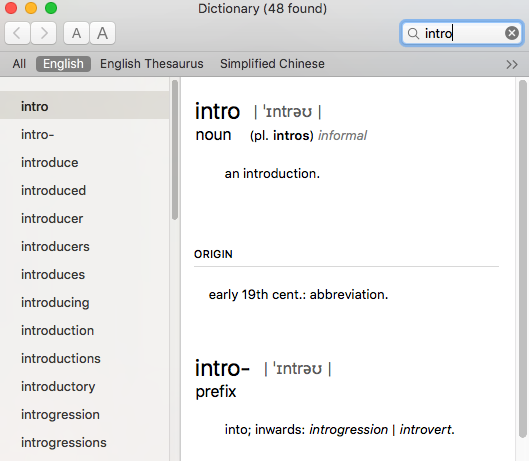
\includegraphics[scale=0.5]{img/edict-en.eps}
  \caption{电子词典。所有和用户输入匹配的候选单词全被列出}
  \label{fig:e-dict}
\end{figure}

电子词典通常存有数十万单词。进行全词查找的开销很大。商业电子词典软件会同时使用多重方法以提高性能,包括缓存(caching)、索引(indexing)等等。

和电子词典类似,图\ref{fig:word-completion}显示了某互联网搜索引擎的界面。当用户输入内容后,会列出一些可能的候选搜索项。这些项的开头部分和用户输入相匹配\footnote{实际功能会更加复杂,包括拼写检查,关键词提取、引导等。},并且按照被搜索的热门程度排序。被搜索的次数越多,越排在前面。

\begin{figure}[htbp]
  \centering
  \includegraphics[scale=0.5]{img/adaptive-input.eps}
  \caption{搜索引擎。和用户输入匹配的候选搜索被列出}
  \label{fig:word-completion}
\end{figure}

这两个例子中,软件都提供了某种自动完成的机制。在某些现代的IDE(集成开发环境)中,编辑器还可以帮助用户自动完成程序代码。

我们看看如何使用前缀树来实现电子词典。为了简化问题,假设我们的词典是英—英词典。

词典中保存了key-value对,key是英文单词或者词组,value是对应的解释。

当用户输入‘a’的时候,词典不是只给出‘a’的意思,而是提供一系列候选单词的列表。这些候选单词都以‘a’开头,包括abandon、about、accent、adam……当然,这些都是存储在前缀树中的单词。

如果候选单词太多,一种方案是只显示前10个,如果用户查找的单词不在其中,他可以浏览更多的候选项。如果待查找的字符串为空,我们从当前节点扩展出前$n$个子节点作为候选项;否则,我们递归地在有共同前缀的子分支中查找。

在支持惰性求值(lazy evaluation)的编程环境中,一种简单直观的方法是惰性扩展全部的子节点,然后根据需要取前$n$个。记前缀树前缀树为$T = (v, C)$,下面的函数枚举所有以$k$开头的内容。

\be
findAll(T, k) = \left \{
  \begin{array}
  {r@{\quad:\quad}l}
  enum(C) & k = \phi, v = \phi \\
  \{(\phi, v)\} \cup enum(C) & k = \phi, v \neq \phi \\
  find(C, k) & k \neq \phi
  \end{array}
\right.
\ee

前两行处理key为空的边界情况。此时,我们通过枚举扩展所有数据不为空的子节点。最后一行调用$find$函数寻找和前缀$k$匹配的子分支。

如果节点的子分支不为空,记$C = \{(k_1, T_1), (k_2, T_2), ..., (k_m, T_m)\}$,令除去第一对映射以外的剩余映射为$C'$。枚举算法可以定义如下:

\be
enum(C) = \left \{
  \begin{array}
  {r@{\quad:\quad}l}
  \phi & C = \phi \\
  mapAppend(k_1, findAll(T_1, \phi)) \cup enum(C')
  \end{array}
\right.
\ee

其中$mapAppend(k, L) = \{(k + k_i, v_i)| (k_i, v_i) \in L\}$。它将前缀$k$添加到列表$L$中的所有key-value对的key前面\footnote{可以进一步抽象为对第一个元素进行映射。在Haskell中,使用范畴论中的箭头概念,$mapAppend$可被表示为$map(first(k+), L)$}。

函数$enum$也可用$concatMap$的概念定义(亦称为$flatMap$)\footnote{效果上相当于先对每个元素进行映射,然后将结果连接起来。通常使用build-foldr来消除中间结果中的列表}。

\be
enum(C) = concatMap(\lambda_{(k, T)} . mapAppend(k, findAll(T, \phi)))
\ee

函数$find(C, k)$定义如下。如果子树为空,结果也为空;否则,它首先检查$k_1$映射的子树$T_1$。如果$k_1$和$k$相等,就调用$mapAppend$向$T_1$所有子分支的key前增加前缀$k$;如果$k_1$是$k$的前缀,算法就递归地查找所有以$k - k_1$开头的子分支;反之,如果$k$是$k_1$的前缀,则$T_1$的所有子分支都是候选项。否则,算法跳过第一对映射,继续处理剩余的其他映射。

\be
find(C, k) = \left \{
  \begin{array}
  {r@{\quad:\quad}l}
  \phi & C = \phi \\
  mapAppend(k_1, findAll(T_1, \phi)) & k \sqsubset k_1 \\
  mapAppend(k_1, findAll(T_1, k - k_1)) & k_1 \sqsubset k \\
  find(C', k) & otherwise
  \end{array}
\right.
\ee

下面的Scala例子程序按照上述算法实现了一个简单的电子词典:

\lstset{language=Scala}
\begin{lstlisting}
def findAll[K, V] (t: PrefixTree.Tree[K, V],
                   key: List[K]): Stream[(List[K], V)] = {
  def enum[K, V] (cs: List[(List[K], PrefixTree.Tree[K, V])]):
    Stream[(List[K], V)] = cs.toStream.flatMap { p =>
                   mapAppend(p._1, findAll(p._2, List()))}
  def find(cs: List[(List[K], PrefixTree.Tree[K, V])],
           key: List[K]): Stream[(List[K], V)] =
    cs match {
      case List() => Stream.empty
      case p :: ps => {
        val (k, tr) = p
        if (k.startsWith(key)) {
          mapAppend(k, findAll(tr, List()))
        } else if (key.startsWith(k)) {
          mapAppend(k, findAll(tr, key.drop(k.length)))
        } else {
          find(ps, key)
        }
      }
    }
  if (key.isEmpty) {
    val ps = enum(t.children)
    if (t.value.isEmpty) ps else (List(), t.value.get) #:: ps
  } else {
    find(t.children, key)
  }
}

def mapAppend[A, B] (a: List[A], ps: Stream[(List[A], B)]):
  Stream[(List[A], B)] = ps.map {p => (a ++ p._1, p._2)}
\end{lstlisting}

在惰性求值编程环境中,前$n$个候选项可以通过$take(n, findAll(T, k))$来获取。附录A给出了$take$函数的详细定义。

\begin{lstlisting}
def lookup[K, V] (t: PrefixTree.Tree[K, V],
                  key: List[K], n: Int): List[(List[K], V)] =
  findAll(t, key).take(n).toList
\end{lstlisting}

也可以用命令式的方式实现电子词典。下面的算法复用了前面定义的前缀树查找函数。当我们找到一个节点,其对应的前缀和用户输入的内容一致时,算法将扩展该节点的所有子树直到获取到前$n$个候选项。

\begin{algorithmic}[1]
\Function{Look-Up}{$T, k, n$}
  \If{$T = $ NIL}
     \State \Return $\phi$
  \EndIf
  \State $prefix \gets$ NIL
  \Repeat
    \State $match \gets$ FALSE
    \For{$\forall (k_i, T_i) \in $ \Call{Children}{$T$}}
      \If{$k$ is prefix of $k_i$}
        \State \Return \Call{Expand}{$prefix + k _i, T_i, n$}
      \EndIf
      \If{$k_i$ is prefix of $k$}
        \State $match \gets$ TRUE
        \State $k \gets k - k_i$
        \State $T \gets T_i$
        \State $prefix \gets prefix + k_i$
        \State break
      \EndIf
    \EndFor
  \Until{$\lnot match$}
  \State \Return $\phi$
\EndFunction
\end{algorithmic}

其中函数\textproc{Expand}($T, prefix, n$)选取$n$个子树,这些子树在$T$中有同样的前缀。它的实现为广度优先遍历(BFS),本书最后一章对包括广度优先在内的搜索算法有详细的介绍。

\begin{algorithmic}[1]
\Function{Expand}{$prefix, T, n$}
  \State $R \gets \phi$
  \State $Q \gets \{(prefix, T)\}$
  \While{$|R| < n \land Q$ is not empty}
    \State $(k, T) \gets$ \Call{Pop}{$Q$}
    \If{\Call{Data}{$T$} $\neq$ NIL}
      \State $R \gets R \cup \{(k, $ \Call{Data}{$T$} $)\}$
    \EndIf
    \For{$\forall (k_i, T_i) \in$ \Call{Children}{$T$} in sorted order}
      \State \Call{Push}{$Q, (k + k_i, T_i)$}
    \EndFor
  \EndWhile
\EndFunction
\end{algorithmic}

下面的Java例子程序实现了一个电子词典。它使用了标准库中的\texttt{find}函数来判断一个字符串是否是另一个的前缀。

\lstset{language=Java}
\begin{lstlisting}
public <T> List<Map.Entry<String, T>> lookup(PrefixTree.Node<T> t,
                                             String key, int n) {
    if (t == null)
        return Collections.emptyList();
    String prefix = "";
    boolean match;
    do {
        match = false;
        for (Map.Entry<String, PrefixTree.Node<T>> entry : t.subTrees.entrySet()) {
            String k = entry.getKey();
            PrefixTree.Node<T> tr = entry.getValue();
            if (k.startsWith(key)) { // key is prefix of k
                return expand(prefix + k, tr, n);
            }
            if (key.startsWith(k)) {
                match = true;
                key = key.substring(k.length());
                t = tr;
                prefix = prefix + k;
                break;
            }
        }
    } while (match);
    return Collections.emptyList();
}

<T> List<Map.Entry<String, T>> expand(String prefix, PrefixTree.Node<T> t, int n) {
    List<Map.Entry<String, T>> res = new ArrayList<>();
    Queue<Map.Entry<String, PrefixTree.Node<T> >> q = new LinkedList<>();
    q.offer(entryOf(prefix, t));
    while(res.size() < n && !q.isEmpty()) {
        Map.Entry<String, PrefixTree.Node<T>> entry = q.poll();
        String s = entry.getKey();
        PrefixTree.Node<T> tr = entry.getValue();
        if (tr.value.isPresent()) {
            res.add(entryOf(s, tr.value.get()));
        }
        for (Map.Entry<String, PrefixTree.Node<T>> e :
                 new TreeMap<>(tr.subTrees).entrySet()) {
            q.offer(entryOf(s + e.getKey(), e.getValue()));
        }
    }
    return res;
}

<K, V> Map.Entry<K, V> entryOf(K key, V val) {
    return new AbstractMap.SimpleImmutableEntry<K, V>(key, val);
}
\end{lstlisting}

%=====================================
% T9
%=====================================

\subsection{T9输入法}
\index{T9}
\index{Textonym输入法}

手机用户编辑短信或者电子邮件时的体验和PC上完全不同。手机键盘(称为ITU-T键盘)上只有非常少的按键。如图\ref{fig:itut-keypad}所示。

\begin{figure}[htbp]
  \centering
  \includegraphics[scale=0.4]{img/itu-t.eps}
  \caption{手机ITU-T键盘}
  \label{fig:itut-keypad}
\end{figure}

在ITU-T键盘上输入英文单词或短语有两种方法。例如用户要输入单词home,他需要按照下面的顺序按键:

\begin{itemize}
\item 按两次4键以输入字符h;
\item 按三次6键以输入字符o;
\item 按一次6键以输入字符m;
\item 按两次3键以输入字符e;
\end{itemize}

另外一种更快速的方法使用下面的按键顺序:

\begin{itemize}
\item 依次按下4、6、6、3,单词home出现在候选列表的最上方;
\item 按下‘*’号键以变换不同的候选单词,good此时出现在候选列表上;
\item 按下‘*’号键再次变换,下一个候选单词gone出现在列表上;
\item ……
\end{itemize}

对比这两个方法,可以发现后者更加方便,但是需要额外保存一个候选单词字典。这种方法被称作“T9输入法”或预测输入法\cite{wiki-t9}、\cite {wiki-predictive-text}。T9是英文textonym的缩写,它以T开头,后面跟9个字母。T9输入法可以用前缀树来实现。

为了向用户提供候选单词,T9输入法需要预先准备一个词典。商业上的T9输入法通常使用更加复杂的索引词典,同时在文件系统和缓存中进行快速索引。本节中的实现仅仅出于演示的目的。

首先我们需要定义T9键盘映射,它将数字映射为候选字符。

\be
\begin{array}{ll}
M_{T9} = \{ & 2 \rightarrow abc, 3 \rightarrow def, 4 \rightarrow ghi, \\
           & 5 \rightarrow jkl, 6 \rightarrow mno, 7 \rightarrow pqrs, \\
           & 8 \rightarrow tuv, 9 \rightarrow wxyz \}
\end{array}
\ee

使用这一映射后,$M_{T9}[i]$就返回数字$i$对应的若干个字符。我们也可以定义从字符到数字的逆映射。

\be
M^{-1}_{T9} = concat(\{\{c \rightarrow d | c \in S\} | (d \rightarrow S) \in M_{T9}\})
\ee

通过查找$M^{-1}_{T9}$,我们可以将字符串转换成一组按键序列。

\be
digits(S) = \{ M^{-1}_{T9}[c]| c \in S \}
\ee


给定一个数字序列$D = d_1d_2...d_n$,我们定义T9查找的算法如下。

\be
findT9(T, D) = \left \{
  \begin{array}
  {r@{\quad:\quad}l}
  \{ \phi \} & D = \phi \\
  concatMap(find, prefixes(T)) & otherwise
  \end{array}
\right.
\ee

其中$T$是从一组单词和词组中构造出的前缀树。我们将其作为T9输入法的词典。若输入的数字串$D$为空,则候选单词的结果列表也是空。否则,我们搜索匹配输入的子树并将结果连接起来。

为了枚举所有匹配的子树,我们检查子树集$C_T$中的每一对$(k_i, T_i)$。首先将字符串$k_i$转换为数字串$d_i$,然后比较$d_i$和$D$。如果其中之一是另一个的前缀,则选中这一对$(k_i, T_i)$进行进一步查找。

\be
prefixes(T) = \{(k_i, T_i) | (k_i, T_i) \in C_T, d_i = digits(k_i), d_i \sqsubset D \lor D \sqsubset d_i \}
\ee

函数$find$接受两个参数,一个前缀$S$和需要进一步查找的子树$T'$。其中$S$是$D$的前缀。为此,我们从$D$中去除这一前缀,然后用剩余的数字串$D' = D - S$继续查找。最后再将$S$添加回递归查找的各个结果前面。

\be
find(S, T') = \{ take(n, S + s_i) | s_i \in findT9(T', D - S) \}
\ee

其中$n = |D|$是输入数字串的长度。函数$take(n, L)$从列表$L$中获取前$n$个元素。如果列表的长度短于$n$,则获取全部元素。

下面的Scala例子程序实现了从前缀树查找的T9输入法。

\lstset{language=Scala}
\begin{lstlisting}
val mapT9 = Map('1' -> ",.", '2' -> "abc", '3' -> "def",
                '4' -> "ghi", '5' -> "jkl", '6' -> "mno",
                '7'-> "pqrs", '8' -> "tuv", '9' -> "wxyz")

val rmapT9 = mapT9.toList.flatMap(p =>
                     p._2.toList.map {(_, p._1)}).toMap

def digits(w: String) = w.map {rmapT9.getOrElse(_, '#')}

def findT9[V](t: Tree[Char, V], key: String): Stream[String] =
  if(key.isEmpty){
    Stream("")
  } else {
    val n = key.length
    val prefixes = t.children.toStream.filter(p => {
      val ds = digits(p._1.mkString)
      ds.startsWith(key) || key.startsWith(ds)
    })
    def find(s: String, tr: Tree[Char, V]): Stream[String] =
      findT9(tr, key.drop(s.length)).map { w => (s ++ w).take(n)}
    prefixes.flatMap { p => find(p._1.mkString, p._2) }
  }
\end{lstlisting}

可以使用广度优先搜索实现命令式的T9输入法。我们使用一个队列$Q$,其保存的元素为三元组
$(prefix, D, T)$。每个三元组包含一个已搜索过的前缀$prefix$,尚未搜索的剩余部分$D$,
还有待搜索的子树$T$。队列初始的时候,三元组包含一个空前缀,全部待搜索的数字,以及前缀树
的根节点。算法不断从队列中取出三元组,对其中的树$T$,依次检查它的子树$T_i$。通过检索
T9的逆映射,我们将子树对应的前缀串$k_i$转换成数字串$D'$。如果$D$是$D'$的前缀,说明
找到了一个候选单词。我们将$k_i$添加到三元组中的前缀$prefix$后,并纪录下这一结果。
如果$D'$是$D$的前缀,我们需要继续在这棵子树中查找。为此,我们将已$k_i$结尾的前缀,
剩余的数字串$D-D'$和该子树组成一个新的三元组,放入队列的尾部。

\begin{algorithmic}[1]
\Function{Look-Up-T9}{$T, D$}
  \State $R \gets \phi$
  \If{$T =$ NIL or $D = \phi$}
    \State \Return $R$
  \EndIf
  \State $n \gets |D|$
  \State $Q \gets \{(\phi, D, T)\}$
  \While{$Q \neq \phi$}
    \State $(prefix, D, T) \gets$ \Call{Pop}{$Q$}
    \For{$\forall (k_i, T_i) \in $ \Call{Children}{$T$}}
      \State $D' \gets$ \Call{Digits}{$k_i$}
      \If{$D' \sqsubset D$} \Comment{$D'$ is prefix of $D$}
        \State $R \gets R \cup \{$ \textproc{Take} $(n, prefix + k_i) \}$ \Comment{限制长度不超过$n$}
      \ElsIf{$D \sqsubset D'$}
        \State \textproc{Push}($Q, (prefix + k_i, D - D', T_i)$)
      \EndIf
    \EndFor
  \EndWhile
  \State \Return $R$
\EndFunction
\end{algorithmic}

函数\textproc{Digits}($S$)将字符串$S$转换为数字串。

\begin{algorithmic}[1]
\Function{Digits}{$S$}
  \State $D \gets \phi$
  \For{each $c \in S$}
    \State $D \gets D \cup \{M^{-1}_{T9}[c]\}$
  \EndFor
  \State \Return $D$
\EndFunction
\end{algorithmic}

下面的Java例子程序使用前缀树实现了T9输入法。

\lstset{language=Java}
\begin{lstlisting}
static final Map<Character, String> MAP_T9 = Map.of('1', ",.",
       '2', "abc", '3', "def", '4', "ghi", '5', "jkl",
       '6', "mno", '7', "pqrs", '8', "tuv", '9', "wxyz");

static final Map<Character, Character> RMAP_T9 = reverseMap();

static Map<Character, Character> reverseMap() {
    Map<Character, Character> m = new HashMap<>();
    for (Character d : MAP_T9.keySet()) {
        String cs = MAP_T9.get(d);
        for (int i = 0; i < cs.length(); ++i)
                m.put(cs.charAt(i), d);
    }
    return m;
}

public static String digits(String w) {
    StringBuilder d = new StringBuilder();
    for(int i = 0; i < w.length(); ++i)
        d.append(RMAP_T9.get(w.charAt(i)));
    return d.toString();
}

static class Tuple<T> {
    String prefix;
    String key;
    Node<T> tree;
    Tuple(String p, String k, Node<T> t) {
        prefix = p; key = k; tree = t;
    }
    public static <T> Tuple<T> of(String prefix, String key,
                                  Node<T> tree) {
        return new Tuple<T>(prefix, key, tree);
    }
}

static String limit(int n, String s) {
    return s.substring(0, Math.min(n, s.length()));
}

public static <T> List<String> lookupT9(Node<T> t, String key) {
    List<String> res = new ArrayList<>();
    if (t == null || key.isEmpty())
        return res;
    Queue<Tuple<T>> q = new LinkedList<>();
    q.offer(Tuple.of("", key, t));
    while (!q.isEmpty()) {
        Tuple<T> elem = q.poll();
        for (Map.Entry<String, Node<T>> e :
                 elem.tree.subTrees.entrySet()) {
            String k = e.getKey();
            String ds = digits(k);
            if (ds.startsWith(elem.key)) {
                res.add(limit(key.length(), elem.prefix + k));
            } else if (elem.key.startsWith(ds)) {
                q.offer(Tuple.of(elem.prefix + k,
                                 elem.key.substring(k.length()),
                                 e.getValue()));
            }
        }
    }
    return res;
}
\end{lstlisting}

\begin{Exercise}
\begin{itemize}
\item 使用Trie实现电子词典和T9输入法。
\item 对于返回多个候选结果的前缀树查找算法,如何保证输出的结果按照字典顺序排序?这会对性能产生怎样的影响?
\item 如果不使用惰性求值,如何实现函数式的电子词典和T9输入法?
\end{itemize}
\end{Exercise}

% ================================================================
%                 Short summary
% ================================================================
\section{小结}

本章一开始介绍了整数Trie和前缀树。基于整数前缀树的映射结构在编译器的实现中得到了重要的应用。字符Trie和字符前缀树可以看做是整数映射结构的自然扩展。它们可以被用来处理文字信息。作为例子,我们介绍了自动预测完成输入的电子词典和T9输入法。尽管和商业软件的实现不同,这些例子展示了如何使用Trie和前缀树来解决问题的方法。某些重要的数据结构,如后缀树和本章中介绍的内容紧密相关。读者可以参考附录E。

\ifx\wholebook\relax\else
\begin{thebibliography}{99}

\bibitem{CLRS}
Thomas H. Cormen, Charles E. Leiserson, Ronald L. Rivest and Clifford Stein.
``Introduction to Algorithms, Second Edition''. Problem 12-1. ISBN:0262032937. The MIT Press. 2001(《算法导论》)

\bibitem{okasaki-int-map}
Chris Okasaki and Andrew Gill. ``Fast Mergeable Integer Maps''. Workshop on ML, September 1998, pages 77-86.  \url{http://www.cse.ogi.edu/~andy/pub/finite.htm}

\bibitem{patricia-morrison}
D.R. Morrison, ``PATRICIA -- Practical Algorithm To Retrieve  Information Coded In Alphanumeric", Journal of the ACM, 15(4), October 1968, pages 514-534.

\bibitem{wiki-suffix-tree}
Suffix Tree, Wikipedia. \url{http://en.wikipedia.org/wiki/Suffix_tree}

\bibitem{wiki-trie}
Trie, Wikipedia. \url{http://en.wikipedia.org/wiki/Trie}

\bibitem{wiki-t9}
T9 (predictive text), Wikipedia. \url{http://en.wikipedia.org/wiki/T9_(predictive_text)}

\bibitem{wiki-predictive-text}
Predictive text,
Wikipedia. \url{http://en.wikipedia.org/wiki/Predictive_text}

\end{thebibliography}

\end{document}
\fi
